%&latexf
\documentclass[]{kclthesis}

%===========================================================
% Change below accordingly and remove``\red{}''
%===========================================================
\modulecode{\red{7CCSMPRJ/7CCSMUIP}} %Use the right module code
\submissiontitle{Individual Project Submission \red{20XX/XX (Replace XX by year)}}
\studentnumber{\red{Student number goes here}}
\programme{\red{Programme title goes here}}
\supervisor{\red{Supervisor's name goes here}}
\wordcount{\red{Word count goes here}}
\title{\red{Project title goes here}}
\author{\red{Your name goes here}}
\ReleaseProject{0} %Replace 0 by 1 if release project; Replace 0 by 2 if not release project
\department{\red{Engineering/Information}} %use the right department
%===========================================================


% nomenclature 
\usepackage[intoc]{nomencl} 
%\makenomenclature
\makeindex
% glossaries
\usepackage[toc, acronym]{glossaries} 
\usepackage{float}
\usepackage{hyperref}
\usepackage[utf8]{inputenc}
\usepackage{graphbox}
\usepackage{hyperref}

\linespread{1}
\newfam\msbfam
\def\Bbb#1{\fam\msbfam\relax#1}

\newtheorem{theorem}{Theorem}[section]
\newtheorem{exa}{Example}[section]
\newtheorem{corollary}[theorem]{Corollary}
\newtheorem{lemma}[theorem]{Lemma}
\newtheorem{proposition}[theorem]{Proposition}

\theoremstyle{definition}
\newtheorem{definition}[theorem]{Definition}
\newtheorem{remark}[theorem]{Remark}
\newtheorem{notation}[theorem]{Notation}
\newtheorem{assumption}[theorem]{Assumption}
\newtheorem{conjecture}[theorem]{Conjecture}

\newcommand{\ind}{1\hspace{-2.1mm}{1}} %Indicator Function
\newcommand{\I}{\mathtt{i}}
\newcommand{\D}{\mathrm{d}}
\newcommand{\E}{\mathrm{e}}
\newcommand{\RR}{\mathbb{R}}
\newcommand{\sgn}{\mathrm{sgn}}
\newcommand{\atanh}{\mathrm{arctanh}}
\def\equalDistrib{\,{\buildrel \Delta \over =}\,}
\numberwithin{equation}{section}
\def\blue#1{\textcolor{blue}{#1}}
\def\red#1{\textcolor{red}{#1}}

\setcounter{tocdepth}{5}
\setcounter{secnumdepth}{5}

% customize your general setup here
%\title{\red{Project title goes here}}
%\author{\red{Your name goes here}}


\begin{document}
\pagenumbering{gobble}


%%%%%% depends what you like, might try out the other frontpage as well
\maketitle 		% official styled layout
\maketitleTwo 	% adapted layout which looks nicer from my point of view.

%%%%%% empty page after main page.
\newpage
\thispagestyle{empty}
\mbox{}
\newpage
%%%%%% Acknowledgements, Abstract, Nomenclature
\section{Template Descriptions}

\subsection{Template Folder Structure}
	After unzip the Latex template, you will find the following folders:
\begin{itemize}
	\item \textbf{``root'' folder:} The file ``thesis.tex'' is the master file of the whole document, which defines the structure of the chapters and other settings.
	\item \textbf{``contents'' folder:}  This is the folder for all chapters. Use the path \begin{verbatim}contents/chapter_filename\end{verbatim} when including chapters. The following files can be found in this folder.
	\begin{itemize}
		\item acknowledgements.tex: the contents of the Acknowledgement chapter. 
		\item abstract.tex: the contents of the Abstract chapter. 
		\item nomenclature.tex: the contents of the Nomenclature chapter. 
		\item introduction.tex: the contents of the Introduction chapter. 
		\item background.tex: the contents of the Background Theories chapter. 
		\item literature.tex: the contents of the literature review.
		\item approach.tex: the contents of the approach section.
		\item results.tex: the contents of the results section. 
		\item conclusion.tex: the contents of the Conclusion chapter. 
		\item app\_1.tex: the contents of the Appendix chapter. 
		\item sample\_1.bib: the bibtex file for references. Remember to run ``bibtex'' to update the list of reference section.
		\item TemplateDescriptions.tex: this is the content of this chapter (Template Description). Remove the line \begin{verbatim} \section{Template Descriptions}

\subsection{Template Folder Structure}
	After unzip the Latex template, you will find the following folders:
\begin{itemize}
	\item \textbf{``root'' folder:} The file ``thesis.tex'' is the master file of the whole document, which defines the structure of the chapters and other settings.
	\item \textbf{``contents'' folder:}  This is the folder for all chapters. Use the path \begin{verbatim}contents/chapter_filename\end{verbatim} when including chapters. The following files can be found in this folder.
	\begin{itemize}
		\item acknowledgements.tex: the contents of the Acknowledgement chapter. 
		\item abstract.tex: the contents of the Abstract chapter. 
		\item nomenclature.tex: the contents of the Nomenclature chapter. 
		\item introduction.tex: the contents of the Introduction chapter. 
		\item background.tex: the contents of the Background Theories chapter. 
		\item literature.tex: the contents of the literature review.
		\item approach.tex: the contents of the approach section.
		\item results.tex: the contents of the results section. 
		\item conclusion.tex: the contents of the Conclusion chapter. 
		\item app\_1.tex: the contents of the Appendix chapter. 
		\item sample\_1.bib: the bibtex file for references. Remember to run ``bibtex'' to update the list of reference section.
		\item TemplateDescriptions.tex: this is the content of this chapter (Template Description). Remove the line \begin{verbatim} \section{Template Descriptions}

\subsection{Template Folder Structure}
	After unzip the Latex template, you will find the following folders:
\begin{itemize}
	\item \textbf{``root'' folder:} The file ``thesis.tex'' is the master file of the whole document, which defines the structure of the chapters and other settings.
	\item \textbf{``contents'' folder:}  This is the folder for all chapters. Use the path \begin{verbatim}contents/chapter_filename\end{verbatim} when including chapters. The following files can be found in this folder.
	\begin{itemize}
		\item acknowledgements.tex: the contents of the Acknowledgement chapter. 
		\item abstract.tex: the contents of the Abstract chapter. 
		\item nomenclature.tex: the contents of the Nomenclature chapter. 
		\item introduction.tex: the contents of the Introduction chapter. 
		\item background.tex: the contents of the Background Theories chapter. 
		\item literature.tex: the contents of the literature review.
		\item approach.tex: the contents of the approach section.
		\item results.tex: the contents of the results section. 
		\item conclusion.tex: the contents of the Conclusion chapter. 
		\item app\_1.tex: the contents of the Appendix chapter. 
		\item sample\_1.bib: the bibtex file for references. Remember to run ``bibtex'' to update the list of reference section.
		\item TemplateDescriptions.tex: this is the content of this chapter (Template Description). Remove the line \begin{verbatim} \include{contents/TemplateDescriptions}\end{verbatim} from ``thesis.tex'' which will remove the Chapter ``Template Descriptions'' from the document.
	\end{itemize}
	Create a new chapter file if necessary.
	\item \textbf{``figures'' folder:} This is the folder for all figures. Use the path \begin{verbatim}contents/figure_filename\end{verbatim} when including figures.
\end{itemize}

contents/sample1
bibtex, run bibtex

\subsection{Student and Project Information}
	The master file of this template is ``thesis.tex''. Change the following lines accordingly in ``thesis.tex'' to include your information.

\begin{verbatim}
%===========================================================
% Change below accordingly and remove``\red{}''
%===========================================================
\modulecode{\red{7CCSMPRJ/7CCSMUIP}} %Use the right module code
\submissiontitle{Individual Project Submission \red{20XX/XX (Replace XX by year)}}
\studentnumber{\red{Student number goes here}}
\programme{\red{Programme title goes here}}
\supervisor{\red{Supervisor's name goes here}}
\wordcount{\red{Word count goes here}}
\title{\red{Project title goes here}}
\author{\red{Your name goes here}}
\ReleaseProject{0} %Replace 0 by 1 if release project; Replace 0 by 2 if not release project
\department{\red{Engineering/Information}} %use the right department
%===========================================================
\end{verbatim}

	Remove the line \begin{verbatim} \include{contents/TemplateDescriptions}\end{verbatim} from ``thesis.tex'' which will remove the Chapter ``Template Descriptions'' from the document.\\
	
	Replace the image ``signature.png'' in the folder ``figures'' by your signature image in ``png'' format.\end{verbatim} from ``thesis.tex'' which will remove the Chapter ``Template Descriptions'' from the document.
	\end{itemize}
	Create a new chapter file if necessary.
	\item \textbf{``figures'' folder:} This is the folder for all figures. Use the path \begin{verbatim}contents/figure_filename\end{verbatim} when including figures.
\end{itemize}

contents/sample1
bibtex, run bibtex

\subsection{Student and Project Information}
	The master file of this template is ``thesis.tex''. Change the following lines accordingly in ``thesis.tex'' to include your information.

\begin{verbatim}
%===========================================================
% Change below accordingly and remove``\red{}''
%===========================================================
\modulecode{\red{7CCSMPRJ/7CCSMUIP}} %Use the right module code
\submissiontitle{Individual Project Submission \red{20XX/XX (Replace XX by year)}}
\studentnumber{\red{Student number goes here}}
\programme{\red{Programme title goes here}}
\supervisor{\red{Supervisor's name goes here}}
\wordcount{\red{Word count goes here}}
\title{\red{Project title goes here}}
\author{\red{Your name goes here}}
\ReleaseProject{0} %Replace 0 by 1 if release project; Replace 0 by 2 if not release project
\department{\red{Engineering/Information}} %use the right department
%===========================================================
\end{verbatim}

	Remove the line \begin{verbatim} \section{Template Descriptions}

\subsection{Template Folder Structure}
	After unzip the Latex template, you will find the following folders:
\begin{itemize}
	\item \textbf{``root'' folder:} The file ``thesis.tex'' is the master file of the whole document, which defines the structure of the chapters and other settings.
	\item \textbf{``contents'' folder:}  This is the folder for all chapters. Use the path \begin{verbatim}contents/chapter_filename\end{verbatim} when including chapters. The following files can be found in this folder.
	\begin{itemize}
		\item acknowledgements.tex: the contents of the Acknowledgement chapter. 
		\item abstract.tex: the contents of the Abstract chapter. 
		\item nomenclature.tex: the contents of the Nomenclature chapter. 
		\item introduction.tex: the contents of the Introduction chapter. 
		\item background.tex: the contents of the Background Theories chapter. 
		\item literature.tex: the contents of the literature review.
		\item approach.tex: the contents of the approach section.
		\item results.tex: the contents of the results section. 
		\item conclusion.tex: the contents of the Conclusion chapter. 
		\item app\_1.tex: the contents of the Appendix chapter. 
		\item sample\_1.bib: the bibtex file for references. Remember to run ``bibtex'' to update the list of reference section.
		\item TemplateDescriptions.tex: this is the content of this chapter (Template Description). Remove the line \begin{verbatim} \include{contents/TemplateDescriptions}\end{verbatim} from ``thesis.tex'' which will remove the Chapter ``Template Descriptions'' from the document.
	\end{itemize}
	Create a new chapter file if necessary.
	\item \textbf{``figures'' folder:} This is the folder for all figures. Use the path \begin{verbatim}contents/figure_filename\end{verbatim} when including figures.
\end{itemize}

contents/sample1
bibtex, run bibtex

\subsection{Student and Project Information}
	The master file of this template is ``thesis.tex''. Change the following lines accordingly in ``thesis.tex'' to include your information.

\begin{verbatim}
%===========================================================
% Change below accordingly and remove``\red{}''
%===========================================================
\modulecode{\red{7CCSMPRJ/7CCSMUIP}} %Use the right module code
\submissiontitle{Individual Project Submission \red{20XX/XX (Replace XX by year)}}
\studentnumber{\red{Student number goes here}}
\programme{\red{Programme title goes here}}
\supervisor{\red{Supervisor's name goes here}}
\wordcount{\red{Word count goes here}}
\title{\red{Project title goes here}}
\author{\red{Your name goes here}}
\ReleaseProject{0} %Replace 0 by 1 if release project; Replace 0 by 2 if not release project
\department{\red{Engineering/Information}} %use the right department
%===========================================================
\end{verbatim}

	Remove the line \begin{verbatim} \include{contents/TemplateDescriptions}\end{verbatim} from ``thesis.tex'' which will remove the Chapter ``Template Descriptions'' from the document.\\
	
	Replace the image ``signature.png'' in the folder ``figures'' by your signature image in ``png'' format.\end{verbatim} from ``thesis.tex'' which will remove the Chapter ``Template Descriptions'' from the document.\\
	
	Replace the image ``signature.png'' in the folder ``figures'' by your signature image in ``png'' format.\end{verbatim} from ``thesis.tex'' which will remove the Chapter ``Template Descriptions'' from the document.
	\end{itemize}
	Create a new chapter file if necessary.
	\item \textbf{``figures'' folder:} This is the folder for all figures. Use the path \begin{verbatim}contents/figure_filename\end{verbatim} when including figures.
\end{itemize}

contents/sample1
bibtex, run bibtex

\subsection{Student and Project Information}
	The master file of this template is ``thesis.tex''. Change the following lines accordingly in ``thesis.tex'' to include your information.

\begin{verbatim}
%===========================================================
% Change below accordingly and remove``\red{}''
%===========================================================
\modulecode{\red{7CCSMPRJ/7CCSMUIP}} %Use the right module code
\submissiontitle{Individual Project Submission \red{20XX/XX (Replace XX by year)}}
\studentnumber{\red{Student number goes here}}
\programme{\red{Programme title goes here}}
\supervisor{\red{Supervisor's name goes here}}
\wordcount{\red{Word count goes here}}
\title{\red{Project title goes here}}
\author{\red{Your name goes here}}
\ReleaseProject{0} %Replace 0 by 1 if release project; Replace 0 by 2 if not release project
\department{\red{Engineering/Information}} %use the right department
%===========================================================
\end{verbatim}

	Remove the line \begin{verbatim} \section{Template Descriptions}

\subsection{Template Folder Structure}
	After unzip the Latex template, you will find the following folders:
\begin{itemize}
	\item \textbf{``root'' folder:} The file ``thesis.tex'' is the master file of the whole document, which defines the structure of the chapters and other settings.
	\item \textbf{``contents'' folder:}  This is the folder for all chapters. Use the path \begin{verbatim}contents/chapter_filename\end{verbatim} when including chapters. The following files can be found in this folder.
	\begin{itemize}
		\item acknowledgements.tex: the contents of the Acknowledgement chapter. 
		\item abstract.tex: the contents of the Abstract chapter. 
		\item nomenclature.tex: the contents of the Nomenclature chapter. 
		\item introduction.tex: the contents of the Introduction chapter. 
		\item background.tex: the contents of the Background Theories chapter. 
		\item literature.tex: the contents of the literature review.
		\item approach.tex: the contents of the approach section.
		\item results.tex: the contents of the results section. 
		\item conclusion.tex: the contents of the Conclusion chapter. 
		\item app\_1.tex: the contents of the Appendix chapter. 
		\item sample\_1.bib: the bibtex file for references. Remember to run ``bibtex'' to update the list of reference section.
		\item TemplateDescriptions.tex: this is the content of this chapter (Template Description). Remove the line \begin{verbatim} \section{Template Descriptions}

\subsection{Template Folder Structure}
	After unzip the Latex template, you will find the following folders:
\begin{itemize}
	\item \textbf{``root'' folder:} The file ``thesis.tex'' is the master file of the whole document, which defines the structure of the chapters and other settings.
	\item \textbf{``contents'' folder:}  This is the folder for all chapters. Use the path \begin{verbatim}contents/chapter_filename\end{verbatim} when including chapters. The following files can be found in this folder.
	\begin{itemize}
		\item acknowledgements.tex: the contents of the Acknowledgement chapter. 
		\item abstract.tex: the contents of the Abstract chapter. 
		\item nomenclature.tex: the contents of the Nomenclature chapter. 
		\item introduction.tex: the contents of the Introduction chapter. 
		\item background.tex: the contents of the Background Theories chapter. 
		\item literature.tex: the contents of the literature review.
		\item approach.tex: the contents of the approach section.
		\item results.tex: the contents of the results section. 
		\item conclusion.tex: the contents of the Conclusion chapter. 
		\item app\_1.tex: the contents of the Appendix chapter. 
		\item sample\_1.bib: the bibtex file for references. Remember to run ``bibtex'' to update the list of reference section.
		\item TemplateDescriptions.tex: this is the content of this chapter (Template Description). Remove the line \begin{verbatim} \include{contents/TemplateDescriptions}\end{verbatim} from ``thesis.tex'' which will remove the Chapter ``Template Descriptions'' from the document.
	\end{itemize}
	Create a new chapter file if necessary.
	\item \textbf{``figures'' folder:} This is the folder for all figures. Use the path \begin{verbatim}contents/figure_filename\end{verbatim} when including figures.
\end{itemize}

contents/sample1
bibtex, run bibtex

\subsection{Student and Project Information}
	The master file of this template is ``thesis.tex''. Change the following lines accordingly in ``thesis.tex'' to include your information.

\begin{verbatim}
%===========================================================
% Change below accordingly and remove``\red{}''
%===========================================================
\modulecode{\red{7CCSMPRJ/7CCSMUIP}} %Use the right module code
\submissiontitle{Individual Project Submission \red{20XX/XX (Replace XX by year)}}
\studentnumber{\red{Student number goes here}}
\programme{\red{Programme title goes here}}
\supervisor{\red{Supervisor's name goes here}}
\wordcount{\red{Word count goes here}}
\title{\red{Project title goes here}}
\author{\red{Your name goes here}}
\ReleaseProject{0} %Replace 0 by 1 if release project; Replace 0 by 2 if not release project
\department{\red{Engineering/Information}} %use the right department
%===========================================================
\end{verbatim}

	Remove the line \begin{verbatim} \include{contents/TemplateDescriptions}\end{verbatim} from ``thesis.tex'' which will remove the Chapter ``Template Descriptions'' from the document.\\
	
	Replace the image ``signature.png'' in the folder ``figures'' by your signature image in ``png'' format.\end{verbatim} from ``thesis.tex'' which will remove the Chapter ``Template Descriptions'' from the document.
	\end{itemize}
	Create a new chapter file if necessary.
	\item \textbf{``figures'' folder:} This is the folder for all figures. Use the path \begin{verbatim}contents/figure_filename\end{verbatim} when including figures.
\end{itemize}

contents/sample1
bibtex, run bibtex

\subsection{Student and Project Information}
	The master file of this template is ``thesis.tex''. Change the following lines accordingly in ``thesis.tex'' to include your information.

\begin{verbatim}
%===========================================================
% Change below accordingly and remove``\red{}''
%===========================================================
\modulecode{\red{7CCSMPRJ/7CCSMUIP}} %Use the right module code
\submissiontitle{Individual Project Submission \red{20XX/XX (Replace XX by year)}}
\studentnumber{\red{Student number goes here}}
\programme{\red{Programme title goes here}}
\supervisor{\red{Supervisor's name goes here}}
\wordcount{\red{Word count goes here}}
\title{\red{Project title goes here}}
\author{\red{Your name goes here}}
\ReleaseProject{0} %Replace 0 by 1 if release project; Replace 0 by 2 if not release project
\department{\red{Engineering/Information}} %use the right department
%===========================================================
\end{verbatim}

	Remove the line \begin{verbatim} \section{Template Descriptions}

\subsection{Template Folder Structure}
	After unzip the Latex template, you will find the following folders:
\begin{itemize}
	\item \textbf{``root'' folder:} The file ``thesis.tex'' is the master file of the whole document, which defines the structure of the chapters and other settings.
	\item \textbf{``contents'' folder:}  This is the folder for all chapters. Use the path \begin{verbatim}contents/chapter_filename\end{verbatim} when including chapters. The following files can be found in this folder.
	\begin{itemize}
		\item acknowledgements.tex: the contents of the Acknowledgement chapter. 
		\item abstract.tex: the contents of the Abstract chapter. 
		\item nomenclature.tex: the contents of the Nomenclature chapter. 
		\item introduction.tex: the contents of the Introduction chapter. 
		\item background.tex: the contents of the Background Theories chapter. 
		\item literature.tex: the contents of the literature review.
		\item approach.tex: the contents of the approach section.
		\item results.tex: the contents of the results section. 
		\item conclusion.tex: the contents of the Conclusion chapter. 
		\item app\_1.tex: the contents of the Appendix chapter. 
		\item sample\_1.bib: the bibtex file for references. Remember to run ``bibtex'' to update the list of reference section.
		\item TemplateDescriptions.tex: this is the content of this chapter (Template Description). Remove the line \begin{verbatim} \include{contents/TemplateDescriptions}\end{verbatim} from ``thesis.tex'' which will remove the Chapter ``Template Descriptions'' from the document.
	\end{itemize}
	Create a new chapter file if necessary.
	\item \textbf{``figures'' folder:} This is the folder for all figures. Use the path \begin{verbatim}contents/figure_filename\end{verbatim} when including figures.
\end{itemize}

contents/sample1
bibtex, run bibtex

\subsection{Student and Project Information}
	The master file of this template is ``thesis.tex''. Change the following lines accordingly in ``thesis.tex'' to include your information.

\begin{verbatim}
%===========================================================
% Change below accordingly and remove``\red{}''
%===========================================================
\modulecode{\red{7CCSMPRJ/7CCSMUIP}} %Use the right module code
\submissiontitle{Individual Project Submission \red{20XX/XX (Replace XX by year)}}
\studentnumber{\red{Student number goes here}}
\programme{\red{Programme title goes here}}
\supervisor{\red{Supervisor's name goes here}}
\wordcount{\red{Word count goes here}}
\title{\red{Project title goes here}}
\author{\red{Your name goes here}}
\ReleaseProject{0} %Replace 0 by 1 if release project; Replace 0 by 2 if not release project
\department{\red{Engineering/Information}} %use the right department
%===========================================================
\end{verbatim}

	Remove the line \begin{verbatim} \include{contents/TemplateDescriptions}\end{verbatim} from ``thesis.tex'' which will remove the Chapter ``Template Descriptions'' from the document.\\
	
	Replace the image ``signature.png'' in the folder ``figures'' by your signature image in ``png'' format.\end{verbatim} from ``thesis.tex'' which will remove the Chapter ``Template Descriptions'' from the document.\\
	
	Replace the image ``signature.png'' in the folder ``figures'' by your signature image in ``png'' format.\end{verbatim} from ``thesis.tex'' which will remove the Chapter ``Template Descriptions'' from the document.\\
	
	Replace the image ``signature.png'' in the folder ``figures'' by your signature image in ``png'' format. %Remove this line after reading
\red{The content of ``Acknowledgements'' is in ``{\textbackslash}contents{\textbackslash}acknowledgements.tex''}

\mbox{}\newline\vspace{10mm} \mbox{}\LARGE
%
{\bf Acknowledgements} \normalsize \vspace{5mm}

It is a short paragraph to thank those whose have contributed to the project work.

\section*{Abstract}

The Abstract is a short, executive summary of your project. This should include a brief description of the project objectives and research question(s) addressed, followed by a brief description of the main contribution(s) of the project, including a summary of the results achieved and the primary conclusions drawn from the work. This should appear on a single page by itself and should be the second page of the report.
\red{The content of ``Nomenclature'' is in ``{\textbackslash}contents{\textbackslash}nomenclature.tex''.} All abbreviations and symbols used in the report must be listed and defined in alphabetic order.

\section*{Nomenclature}
$a$ \qquad The number of angels per unit area\\
$A$ \qquad The area of the needle point\\
$c$ \qquad Speed of light in a vacuum inertial frame\\
$h$ \qquad Planck constant\\
LMI	\qquad Linear Matrix Inequalities\\
$N$ \qquad The number of angels per needle point

%%%%%% Table of contents

\pagenumbering{roman}
\setcounter{tocdepth}{4}
\tableofcontents
\newpage
%%%%%%%%%%%%%%%%%%%%%%%%%%%%%%%%%%%%%%%%%%%%%%%%%%%%
\thispagestyle{empty}
 
\listoffigures
 
\listoftables
 
\newpage
\fancyhead{}
\fancyfoot{}
\pagestyle{fancy} 
%\fancyhead{\sffamily\small \thepage}
%\fancyhead{\sffamily\small \nouppercase{\rightmark}}
\fancyhead[RO,LE]{\sffamily\small \thepage}
\fancyhead[LO,RE]{\sffamily\small \nouppercase{\rightmark}}
\renewcommand{\headrulewidth}{0.4pt}
\renewcommand{\footrulewidth}{0.0pt}
%%%%%%%%%%%%%%%%%%%%%%%%%%%%%%%%%%%%%%%%%%%%%%%%%%%%

%%%%%% Main content
\pagenumbering{arabic}

%Insert if necessary if more chapters are needed by creating a new .tex file in the folder ``contents'' and use \include{filename} to include the new chapter.
%Modify the section headings if necessary
%Insert more sections if necessary
\section{Introduction}

The Introduction is the first content section of your report. You should describe the general area (e.g., application domain) in which your project research is conducted, the motivation for conducting the research and the overall aims of the research. Be sure to outline your research questions and give a brief summary of the conclusions drawn, though the conclusions will be detailed later in the report. With the Introduction, you want to interest your reader and tell them why they should care about your research and why they should read the rest of the report. The report will be read (marked) by examiners with a technical Computer Science background, but not necessarily any knowledge of your domain, so make sure that you provide enough information for a naive reader.

\red{The content of ``Background'' is in ``{\textbackslash}contents{\textbackslash}background.tex''}

\section{Background Theories} 

The background theories supporting the work should be given in this section. Provide references when someone's work is recalled.
\red{The content of ``Main results'' is in ``{\textbackslash}contents{\textbackslash}introduction.tex''}

The chapter reports the contributions of your work.  For example, it could contain the following sub-sections to summarise the contribution of the project such as Theoretical Development, Analysis and Design, Implementation and Experimental Work, Results, Observation and Discussion.

\section{Objectives, Specification and Design}

	It recalls the objectives in a more detailed way to justify the development of a set of requirements and specifications, and identify a coherent set of issues to be addressed. It explains in detail the design and how the design can achieve the project aim (solve the problem).

\section{Methodology and Implementation}

	It presents and justifies the methodology used to deal with the problem and describes in detail the implementation procedures. The background theory presented in the previous chapter can be recalled to support the proposed implementation. The originality, novelty and contribution are to be demonstrated with the discussion of the strengths and limitations.


\section{Results, Analysis and Evaluation}
	It summarises the results obtained from the proposed design and methodology. The way to obtain the results should be described in detail. Analysis and evaluation have to be performed. Comparisons should be made. It should justifies if the project aims, objectives, requirements and specifications have been achieved.


\section{Others}
\subsection{Maths}
\begin{equation}\label{eq:BS}
\frac{\D S_t}{S_t} = r \D t + \sigma \D W_t,
\qquad S_0>0,
\end{equation}

The equation $\sigma = m a$ follows easily~\cite{Doe11}.


\subsection{Glossary and acronyms}

\Glspl{Linux} and other Unix operating systems are better then Windows because they support \gls{lvm} out of the box~\cite{Joh11}\insertref{A ref is missing here}. 

\subsection{Figures}
Here is an example~\cite{JohSil05} of how to insert a picture:

\begin{figure}[!ht]
\centering
\subfigure{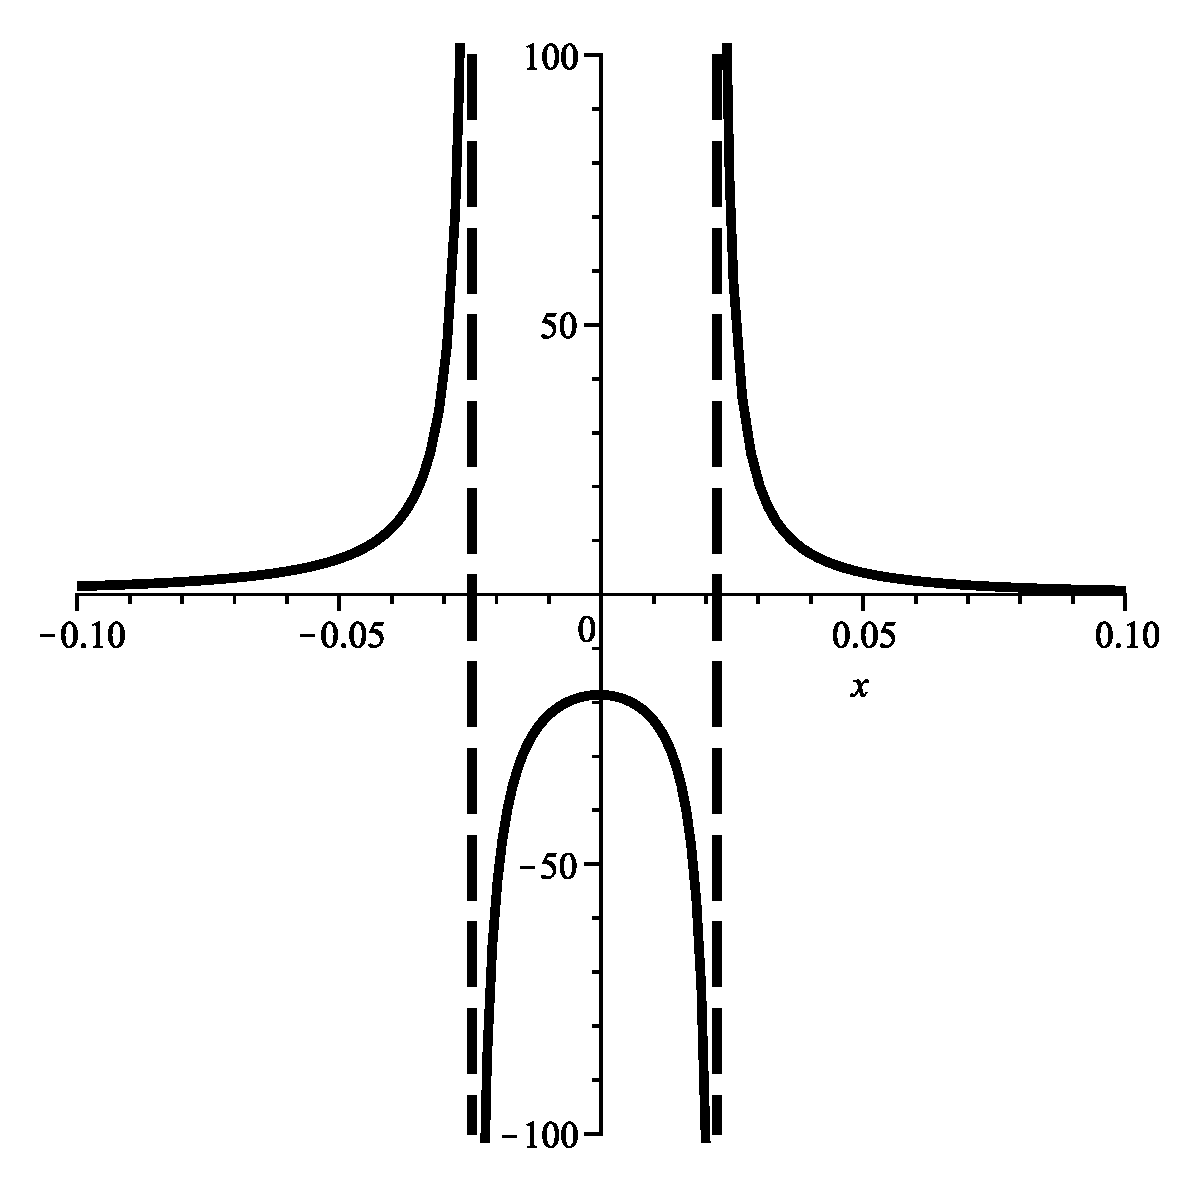
\includegraphics[scale=0.2]{figures/Picture.eps}}
\caption{This is the caption for the figure.}
\label{fig:Pict}
\end{figure}


\begin{figure}[!ht]
\centering
\missingfigure{If you know there will be a figure, but you still need to create it.}
\caption{This is the caption for the figure which is not even present.}
\label{fig:PictMis}
\end{figure}


Lorem ipsum dolor sit amet, consetetur sadipscing elitr, sed diam nonumy eirmod tempor invidunt ut labore et dolore magna aliquyam erat, sed diam voluptua. At vero eos et accusam et justo duo dolores et ea rebum. Stet clita kasd gubergren, no sea takimata sanctus est Lorem ipsum dolor sit amet. Lorem ipsum dolor sit amet, consetetur sadipscing elitr, sed diam nonumy eirmod tempor invidunt ut labore et dolore magna aliquyam erat, sed diam voluptua. At vero eos et accusam et justo duo dolores et ea rebum. Stet clita kasd gubergren, no sea takimata sanctus est Lorem ipsum dolor sit amet.\todo{This is a small Todo, please take care!}

or two side-by-side pictures:

\begin{figure}[!ht]
\centering
\subfigure{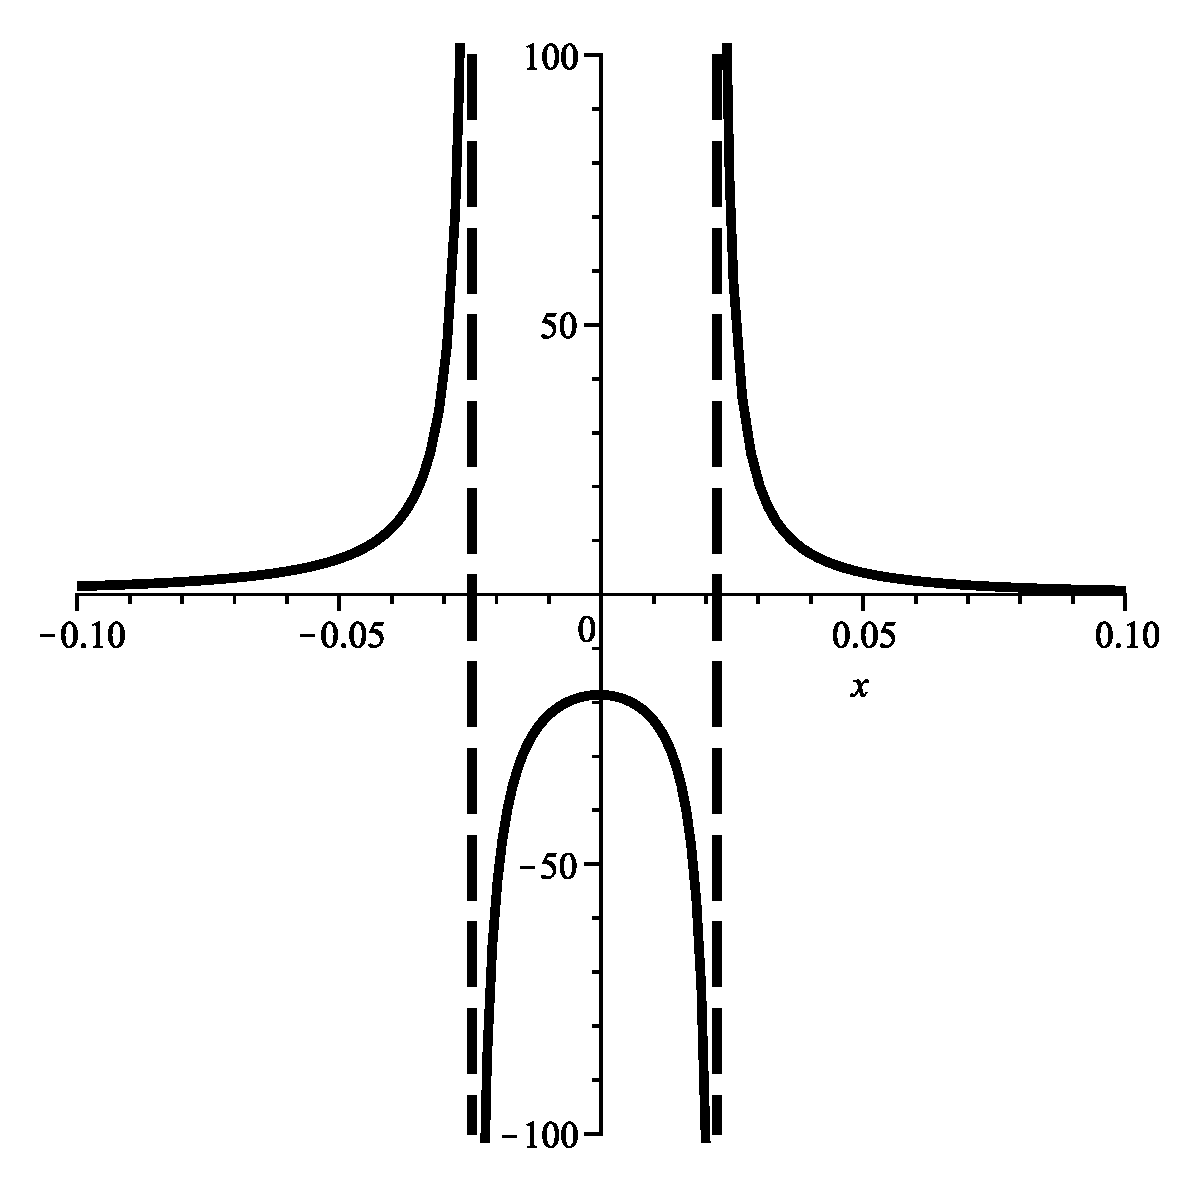
\includegraphics[scale=0.3]{figures/Picture.eps}}
\hspace{15pt}
\subfigure{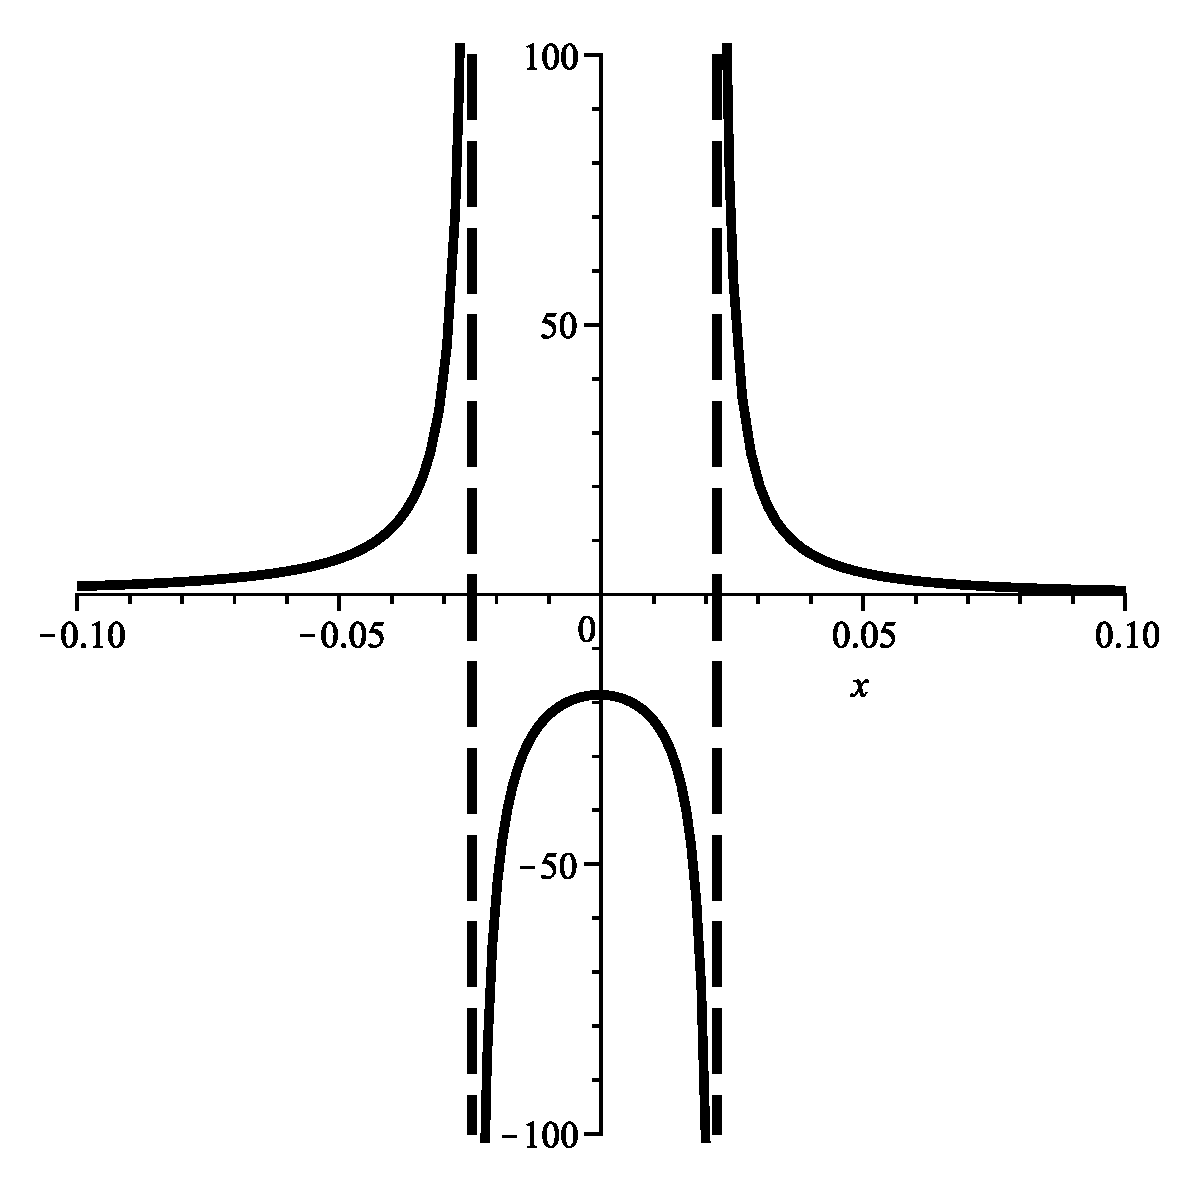
\includegraphics[scale=0.3]{figures/Picture.eps}}

\caption{Another caption}
\label{fig:Pict2}
\end{figure}



\subsection{Table}
Lorem ipsum dolor sit amet, consetetur sadipscing elitr, sed diam nonumy eirmod tempor invidunt ut labore et dolore magna aliquyam erat, sed diam voluptua. At vero eos et accusam et justo duo dolores et ea rebum. Stet clita kasd gubergren, no sea takimata sanctus est Lorem ipsum dolor sit amet. Lorem ipsum dolor sit amet, consetetur sadipscing elitr, sed diam nonumy eirmod tempor invidunt ut labore et dolore magna aliquyam erat, sed diam voluptua. At vero eos et accusam et justo duo dolores et ea rebum. Stet clita kasd gubergren, no sea takimata sanctus est Lorem ipsum dolor sit amet\explainindetail{This needs further explanation}.
\begin{table}[!ht]
	\centering
	\begin{tabular}{|l|rl|}
		\hline
		Something & Someother & Thing \\
  		Seems & to be & good\\
  		\hline
  	\end{tabular}
  	\caption{Random data for a table.}
\end{table}

Lorem ipsum dolor sit amet, consetetur sadipscing elitr, sed diam nonumy eirmod tempor invidunt ut labore et dolore magna aliquyam erat, sed diam voluptua. At vero eos et accusam et justo duo dolores et ea rebum. Stet clita kasd gubergren, no sea takimata sanctus est Lorem ipsum dolor sit amet. Lorem ipsum dolor sit amet, consetetur sadipscing elitr, sed diam nonumy eirmod tempor invidunt ut labore et dolore magna aliquyam erat, sed diam voluptua. At vero eos et accusam et justo duo dolores et ea rebum. Stet clita kasd gubergren, no sea takimata sanctus est Lorem ipsum dolor sit amet.


\section{More Others}
\subsection{What is calibration?}
Here is an example of a matrix\cite{website:fermentas-lambda} in $A\in\mathcal{M}_n(\RR)$:
$$
A = 
\begin{pmatrix}
a_{11} & a_{12} & \ldots & a_{1n}\\
a_{21} & \ddots & \ddots  & \vdots\\
\vdots &  \ddots & \ddots  & \vdots\\
a_{n1} &  \ldots &  \ldots & a_{1n}.
\end{pmatrix}
$$

\subsection{Numerical methods for calibration}
...



\red{The content of ``Conclusion'' is in ``{\textbackslash}contents{\textbackslash}conclusion.tex''}

\section{Conclusion}
	It is a chapter to sum up the main points and findings of the work; how you achieve the project aims and address the research questions; the contributions and results you have achieved.  Future plan and development can be mentioned in this section as well. It is normally in one or two pages.

%%%%% References
\bibliographystyle{ieeetr}
\bibliography{contents/sample1} 
%%%%% Declaration
%\include{structure/declaration}

%%%%% Appendix 
%Insert more section if necessary if more appendix sections are needed
%Remove or remark the following two lines if appendix is not necessary
\appendix
\red{The content of ``Appendix'' is in ``{\textbackslash}contents{\textbackslash}app\_1.tex''}

\section{Appendix}
	Supplementary materials (such as source code, user menu, etc) could be included. Each appendix must be labelled (for example, Appendix A, Appendix A.1, Appendix A.2,  Appendix B, Appendix B.1, etc.) and with heading.  All Appendices must be referred in the text.  

\subsection{Points to Note}
Please note the following points when you write your report:
\begin{itemize}
	\item Consider the outline of the report.  It is a good idea to start with the table of contents, which gives you an overall structure of the report.
	\item Show understanding of the topic and demonstrate the contribution of the work. 70\% of the content of the report should be your own contributions and achievements.
	\item Always use your own words.
	\item The main report and any appendices must constitute one document.
	\item Pages must be numbered consecutively.
	\item Captions must be provided for all figures and tables.
	\item Equations (or important equations), figures and tables must be numbered.
	\item All figures and tables must be referred to in the text.
	\item Units of all variables must be provided.
	\item Numerical values (floating-point number) should be in 4 decimal places.
	\item Contractions should not be used.
	\item Check the punctuation of sentences.  In particular, those sentences with equation.  For example, if an equation is at the end of a sentence, a full stop should be used.
	\item All variables must be defined.
	\item Font face of variables throughout the report (in the text, equation, figures and table) must be consistent.
	\item Use proper headings for chapters, sections, subsections.
	\item Chapters, sections, subsections should be numbered and with the same numbering system throughout the report.
It is suggested that vector and matrix variables should be in bold, scalar variables should be in italic.
	\item References must be used for materials used in the report that are not yours.
	\item A standard reference format must be adopted and be consistently applied through the report.  General guidelines for reference format can be found on KEATS.
	\item Always backup your files.  
\end{itemize}

\section{Review of stochastic calculus}
\subsection{Riemann integration}
\subsection{The It\^o integral}



%%%%%%%%%%%%%%%%%%%%%%%%%%%%%%%%%%%%%%%%%%%%%%%%%%%%
%%%%%%%%%%%%%%%%%%%%%%%%%%%%%%%%%%%%%%%%%%%%%%%%%%%%
%%%%%%%%%%%%%%%%%%%%%%%%%%%%%%%%%%%%%%%%%%%%%%%%%%%%
%%%%%%%%%%%%%%%%%%%%%%%%%%%%%%%%%%%%%%%%%%%%%%%%%%%%


\end{document}
